\documentclass[miniframe]{lbpbeamer}
%\documentclass[handout]{lbpbeamer}
%%%%%%%%%%%%% option de la classe lbpbeamer.cls
% toutes les options standards de la classe beamer
% le type d'en-tete pour l'appel des sections : 
%  - default : currentsection | currentsubsection
%  - miniframe : sections + puces
%  - tree : sections + currentsubsection
%  - split : sections + subsections
%%%%%%%%%%%%%%%%%%%%%%%%%%%%%%%%%%%%%%%%%%%%%%%%%%

%%%%%%%%%%%%% appel des packages
\usepackage[english,french]{babel}
\usepackage{epsfig}
\usepackage[T1]{fontenc}
\usepackage[utf8]{inputenc}
\usepackage{lmodern} 
\usepackage{times}
\usepackage{multirow}
\usepackage{animate}
\usepackage{hyperref}
\usepackage{movie15}
\usepackage{wasysym}
\usepackage[squaren, Gray, cdot]{SIunits}
\usepackage{tikz}
\usetikzlibrary{calc,trees,positioning,arrows,arrows.meta,chains,shapes.geometric,%
	decorations.pathreplacing,decorations.pathmorphing,shapes,%
matrix,shapes.symbols,plotmarks,decorations.markings,shadows}

\usepackage{tabularx}
\newcolumntype{L}[1]{>{\raggedright\let\newline\\\arraybackslash\hspace{0pt}}m{#1}}
\newcolumntype{C}[1]{>{\centering\let\newline\\\arraybackslash\hspace{0pt}}m{#1}}
\newcolumntype{R}[1]{>{\raggedleft\let\newline\\\arraybackslash\hspace{0pt}}m{#1}}

\newcommand{\backupbegin}{
	\newcounter{framenumberappendix}
	\setcounter{framenumberappendix}{\value{framenumber}}
}
\newcommand{\backupend}{
	\addtocounter{framenumberappendix}{-\value{framenumber}}
	\addtocounter{framenumber}{\value{framenumberappendix}} 
}

%\usepackage{enumitem}

%%%%%%%%%%%%%%%%%%%%%%%%%%%%%%%%%%%%%%%%%%%%%%%%%%
%\newlist{fleche}{itemize}{1}
%\setlist[fleche]{label=$\rightarrow$,font=\color{blue}}


%\newcommand{\smiley}{\tikz[baseline=-0.75ex,black]{
%		    \draw circle (2mm);
%			\node[fill,circle,inner sep=0.5pt] (left eye) at (135:0.8mm) {};
%			\node[fill,circle,inner sep=0.5pt] (right eye) at (45:0.8mm) {};
%			\draw (-145:0.9mm) arc (-120:-60:1.5mm);
%			    }
%			}

\newcommand{\orto}{^{\circ}}

%%%%%%%%%%%%% appel du plan a chaque subsection
%% en 1 colonne

%\AtBeginSection[]{
%	\frame{%<handout:0>{
%	\frametitle{Plan}
%  \begin{columns}[t]
%  \begin{column}{0.5\linewidth}
%  \tableofcontents[sections={1-3}, currentsection,subsectionstyle=show/show/shaded]
%  \end{column}
%  \begin{column}{0.5\linewidth}
%  \tableofcontents[sections={4-6}, currentsection,subsectionstyle=show/show/shaded]
%  \end{column}
%  \end{columns}
%  }
%}

%% ou en 2 colonnes s'il y a trop de sections
    
%\AtBeginSubsection[]{
%	\frame{%<handout:0>{
%	\frametitle{Summary}
%  \begin{columns}[t]
%  \begin{column}{0.5\linewidth}
%  \tableofcontents[sections={1-6},currentsection, subsectionstyle=show/shaded/hide]
%  \end{column}
%  \begin{column}{0.5\linewidth}
%  \tableofcontents[sections={7-12},currentsection,subsectionstyle=show/shaded/hide]
%  \end{column}
%  \end{columns}
%  }
%}	
%%%%%%%%%%%%%%%%%%%%%%%%%%%%%%%%%%%%%%%%%%%%%%%%%%	

%%%%%%%%%%%%% Pour supprimer les symboles de navigation
\setbeamertemplate{navigation symbols}{}
%%%%%%%%%%%%%%%%%%%%%%%%%%%%%%%%%%%%%%%%%%%%%%%%%%

%%%%%%%%%%%%% Personnalisation des theoremes
\newtheorem{theoreme}{Th\'eor\`eme}
\newtheorem{preuve}{D\'emonstration}
\newtheorem{define}{D\'efinition}
%%%%%%%%%%%%%%%%%%%%%%%%%%%%%%%%%%%%%%%%%%%%%%%%%%	
		
%%%%%%%%%%%%% Infos personnelles au document	
\title[Présentation SI]{Sciences de l'Ingénieur}
\subtitle{Enseignements d'exploration classe de seconde}
\author[Fiack]{Laurent Fiack}
%\email{}
\institute[Lycée Blaise Pascal]{Lycée Blaise Pascal}
\date[\today]{\today}
\logo{
\includegraphics[scale=0.3]{./figures/logo_si.png}\hspace{1em}}
%%%%%%%%%%%%%%%%%%%%%%%%%%%%%%%%%%%%%%%%%%%%%%%%%%

\newcommand{\figpath}{figures/}

\usepackage{scrextend}

\begin{document}

%%%%%%%%%%%%% Background des slides	
\usebackgroundtemplate{}
%% cet option permet d'ins\'erer une image en fond-ecran
%% la commande \usebackgroundtemplate{} permet de
%% supprimer le fond a partir du moment ou il est 
%% appele
%%%%%%%%%%%%%%%%%%%%%%%%%%%%%%%%%%%%%%%%%%%%%%%%%%	

%%%%%%%%%%%%% frame title
\frame{\titlepage}
\usebackgroundtemplate{}
\logo{}
%\logoheader{taille}{emplacement-image}
%% on supprime les logos des autres frames		
%%%%%%%%%%%%%%%%%%%%%%%%%%%%%%%%%%%%%%%%%%%%%%%%%%
\section[SI]{Sciences de l'Ingénieur}
\subsection[SI]{Sciences de l'Ingénieur}

\frame{
	\frametitle{Sciences de l'ingénieur}
	\scriptsize
	\begin{minipage}[b]{0.55\linewidth}
		\onslide<3->{
		\begin{block}{Objectifs}
			\begin{itemize}
				\item Découvrir comment un produit répond à un besoin et comment il fonctionne.
					\begin{itemize}
							\tiny
						\item Conception et modélisation des solutions avec des démarches scientifique et technologique
						\item Réalisation de solutions
					\end{itemize}
			\end{itemize}
		\end{block}
		}
		\onslide<4->{
		\begin{block}{Apprentissages}
			\begin{itemize}
				\item Approfondir sa culture technologique
				\item Représenter – Communiquer
				\item Simuler, mesurer un comportement
			\end{itemize}
		\end{block}
		}
	\end{minipage}
	\hfill
	\begin{minipage}[b]{0.40\linewidth}
		\onslide<2->{
		\begin{center}
			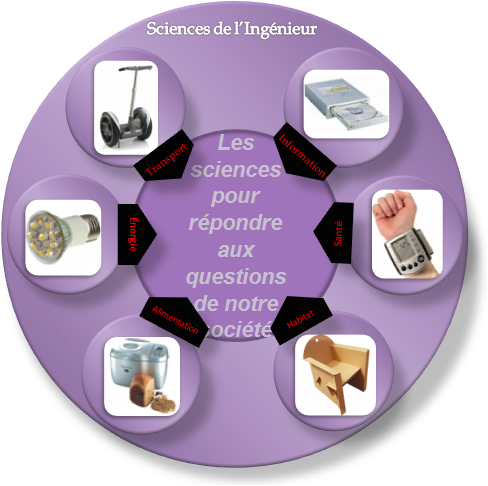
\includegraphics[width=\linewidth]{./figures/si1.png}
		\end{center}
		}
	\end{minipage}

	\onslide<5->{
	\begin{block}{Problématique}
		\textbf{Pourquoi} et \textbf{comment} un produit, à un moment donné, est \textbf{conçu} et \textbf{réalisé}? À quel besoin il répond?

		Quel est son impact sur la \textbf{société} et l'\textbf{environnement}?
	\end{block}
	}
}

\section[Projet]{Challenge robotique}
\subsection[Projet]{Challenge robotique}
\frame{
	\frametitle{Challenge robotique}
	\begin{center}
		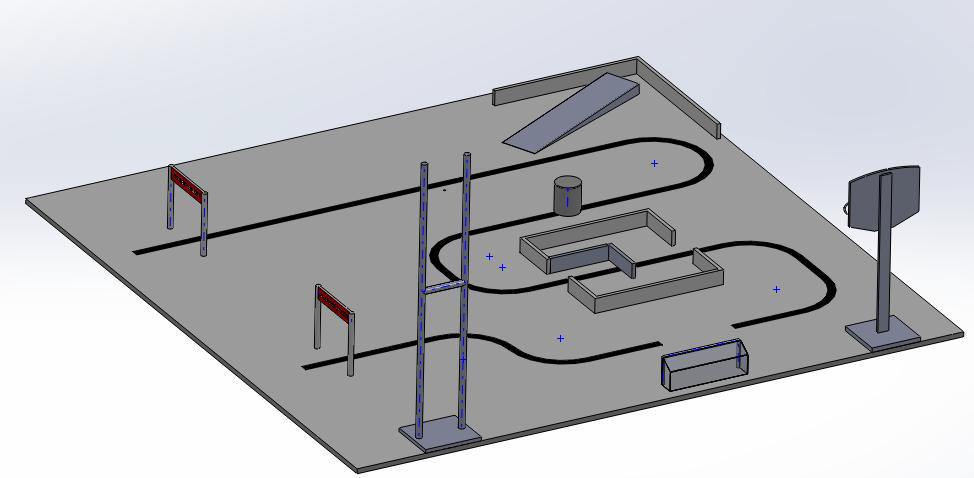
\includegraphics[width=.7\linewidth]{./figures/challenge1.png}
	\end{center}
	\small
	\begin{block}{Défi}
		Construire un \textbf{robot autonome} capable de se déplacer et de faire des actions sur une aire de jeu.

		Le robot doit remporter un maximum de points dans un temps imparti.
	\end{block}
}

\frame{
	\frametitle{Étude d'un produit}
	\begin{center}
		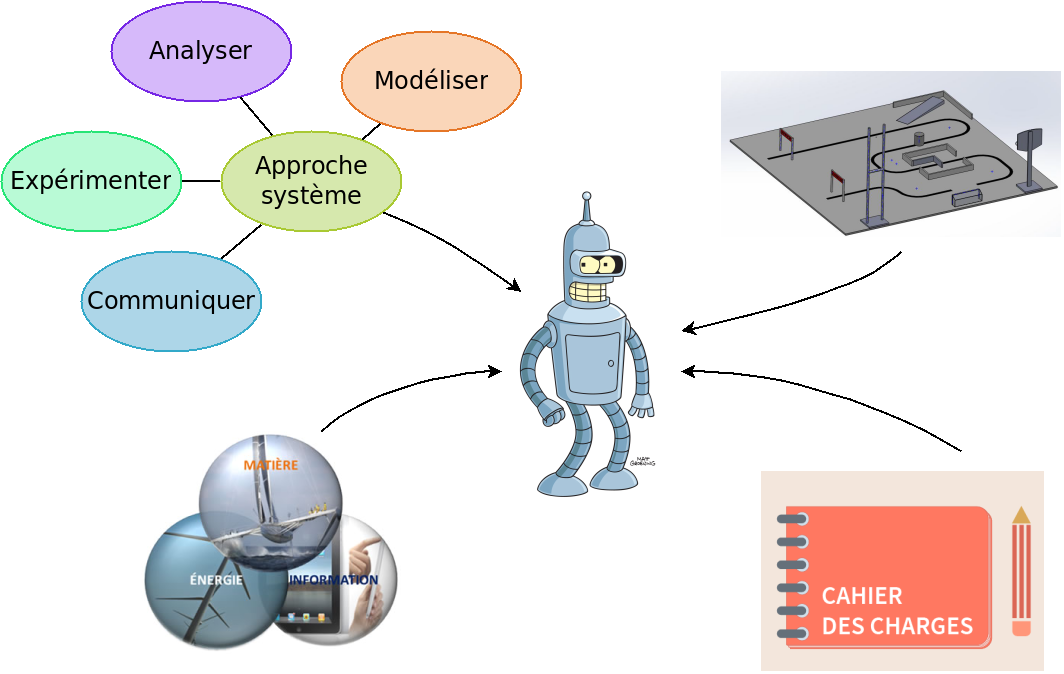
\includegraphics[width=.9\linewidth]{./figures/challenge2.png}
	\end{center}
}

\section[Organisation]{Organisation des activités}
\subsection[Organisation]{Organisation des activités}
\frame{
	\frametitle{Organisation}
	\begin{minipage}[b]{0.48\linewidth}
		\footnotesize
		\begin{block}{Organisation des activités}
			\begin{itemize}
				\item Travaux collectifs et individuels
				\item En îlots
				\item Ordinateur et matériel
			\end{itemize}
		\end{block}
	\end{minipage}
	\hfill
	\begin{minipage}[b]{0.48\linewidth}
		\footnotesize
		\begin{block}{Activités}
			\begin{itemize}
				\item Investigation
				\item Expérimentation virtuelle ou matérielle
				\item Préparation exposé
			\end{itemize}
		\end{block}
	\end{minipage}
	\begin{center}
		Déroulement des séances\\

		
\includegraphics[scale=0.35]{./figures/seance.png}

		Déroulement des activités\\

		
\includegraphics[scale=0.35]{./figures/activite.png}
	\end{center}
}

\frame{
	\frametitle{Vie de classe et matériel}
	\begin{center}
		
\includegraphics[width=.7\linewidth]{./figures/classe.png}
	\end{center}
	\begin{block}{1 classeur}
		\begin{itemize}
			\item Des intercalaires
			\item Des pochettes transparentes
			\item Des feuilles perforées
		\end{itemize}
	\end{block}
}

\frame{
	\frametitle{Apprentissages visés et évaluation}
	\begin{center}
		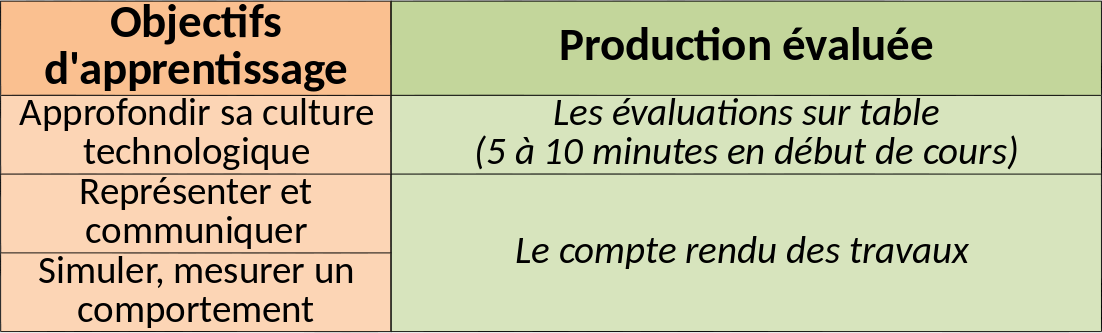
\includegraphics[width=.7\linewidth]{./figures/eval.png}
	\end{center}
}

\end{document}


